\section{Conclusion}

\subsection{Esquisse du futur système}

\begin{center}
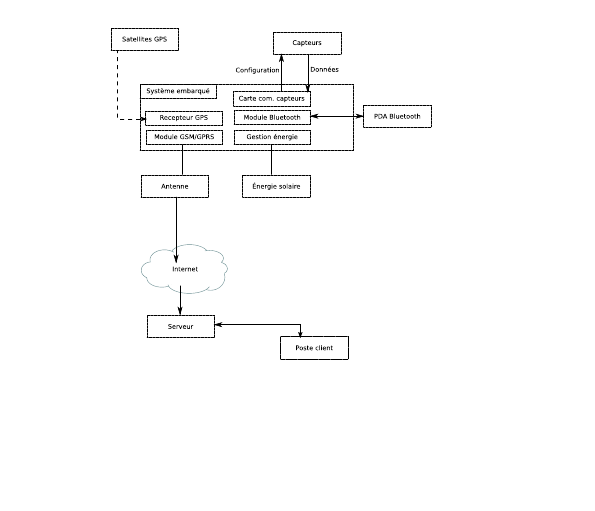
\includegraphics[scale=0.8]{\PIXPATH/schema_archi}
\end{center}
% tel que vous l'envisagez avant de faire la conception et impacts de votre 
% solution

\subsection{Bilan des améliorations}

\section{Bilan des Améliorations}

Les principaux axes d'améliorations sont repris par les spécifications
fonctionnelles. Le tableau présenté ci-dessous décrit le nombre de
spécification unitaire reprennant nos axes d'améliorations. 

Comme mentionné sur la définition des axes d'amélioration, on va que
l'optimisation des coûts se fera conjointement avec l'application des axes
d'améliorations principaux (\textit{En gras sur le tableau})

\begin{center}
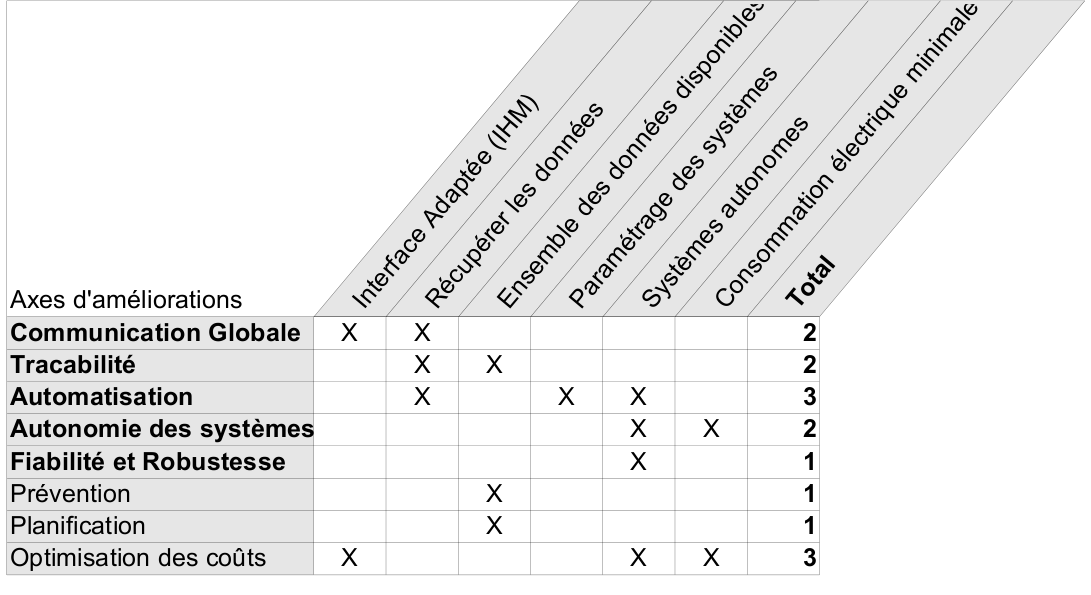
\includegraphics[scale=0.4]{\PIXPATH/amelioration.png}
\end{center}



